\documentclass[handout]{beamer}
\setbeamertemplate{footline}[frame number]
%\documentclass{beamer}

\usepackage[utf8x]{inputenc}
\usepackage[brazil,british]{babel}
\usetheme{default} 
\usecolortheme{beaver}
\newtranslation[to=brazil]{Theorem}{Teorema}
\newtranslation[to=brazil]{Definition}{Definição}
\newtranslation[to=brazil]{Example}{Exemplo}
\newtranslation[to=brazil]{Problem}{Exercício}
\newtranslation[to=brazil]{Solution}{Resolução}
\logo{
\includegraphics[width=1cm]{../img/logo-ppgsc-icon-text.png}}

\usepackage{graphicx}
\usepackage{clrscode3e}
\usepackage{hyperref}

\usepackage{pgf}
\usepackage{tikz}
\newcommand{\assert}[1]{\textcolor{blue}{#1}}



\usepackage{pgf}
\usepackage{tikz}

\title{Aula 05: Análise matemática de algoritmos não recursivos}
\author{David Déharbe \\
  Programa de Pós-graduação em Sistemas e Computação \\
  Universidade Federal do Rio Grande do Norte \\
  Centro de Ciências Exatas e da Terra \\
  Departamento de Informática e Matemáica Aplicada}
\date{}

\begin{document}
\selectlanguage{brazil}
\begin{frame}
  \titlepage
\end{frame}

\begin{frame}
  \frametitle{Plano da aula}
  \tableofcontents
\end{frame}

\section{Introdução}

\begin{frame}

  \frametitle{Contexto}

  \begin{center}
  \begin{pgfpicture}{0cm}{0cm}{9cm}{7.3cm}
  \pgfsetendarrow{\pgfarrowtriangle{3pt}}

  \pgfrect[stroke]{\pgfxy(2,6.5)}{\pgfxy(5,.8)}
  \pgfputat{\pgfxy(4.5,6.9)}{\pgfbox[center,center]{Entender problema}}
  \pgfline{\pgfxy(4.5,6.5)}{\pgfxy(4.5,6.0)}

  \pgfrect[stroke]{\pgfxy(2,5.2)}{\pgfxy(5,.8)}
  \pgfputat{\pgfxy(4.5,5.6)}{\pgfbox[center,center]{Escolher abordagem}}
  \pgfline{\pgfxy(4.5,5.2)}{\pgfxy(4.5,4.7)}

  \pgfrect[stroke]{\pgfxy(2,3.9)}{\pgfxy(5,.8)}
  \pgfputat{\pgfxy(4.5,4.3)}{\pgfbox[center,center]{Projetar algoritmo}}
  \pgfline{\pgfxy(4.5,3.9)}{\pgfxy(4.5,3.4)}

  \pgfrect[stroke]{\pgfxy(2,2.6)}{\pgfxy(5,.8)}
  \pgfputat{\pgfxy(4.5,3.0)}{\pgfbox[center,center]{Provar correção}}
  \pgfline{\pgfxy(4.5,2.6)}{\pgfxy(4.5,2.1)}
  \pgfmoveto{\pgfxy(2.0,3.0)}
  \pgfcurveto{\pgfxy(1.5,3.0)}{\pgfxy(1.5,4.3)}{\pgfxy(2.0,4.3)}
  \pgfstroke
  \pgfmoveto{\pgfxy(2.0,3.0)}
  \pgfcurveto{\pgfxy(1.0,3.0)}{\pgfxy(1.0,5.6)}{\pgfxy(2.0,5.6)}
  \pgfstroke

  \pgfsetcolor{lightgray}
  \pgfrect[fill]{\pgfxy(2,1.3)}{\pgfxy(5,.8)}
  \pgfsetcolor{black}
  \pgfputat{\pgfxy(4.5,1.7)}{\pgfbox[center,center]{Analizar complexidade}}
  \pgfline{\pgfxy(4.5,1.3)}{\pgfxy(4.5,0.8)}
  \pgfmoveto{\pgfxy(7.0,1.7)}
  \pgfcurveto{\pgfxy(7.5,1.7)}{\pgfxy(7.5,4.3)}{\pgfxy(7.0,4.3)}
  \pgfstroke
  \pgfmoveto{\pgfxy(7.0,1.7)}
  \pgfcurveto{\pgfxy(8.0,1.7)}{\pgfxy(8.0,5.6)}{\pgfxy(7.0,5.6)}
  \pgfstroke

  \pgfrect[stroke]{\pgfxy(2,0)}{\pgfxy(5,.8)}
  \pgfputat{\pgfxy(4.5,0.4)}{\pgfbox[center,center]{Codificar algoritmo}}
\end{pgfpicture}
  \end{center}
\end{frame}


\begin{frame}

  \frametitle{Estrutura da apresentação}

  \begin{enumerate}
  \item arcabouço teórico;
  \item melhor caso, pior caso, caso médio;
  \item notações asintóticas; $O$, $\Omega$, $\Theta$;
  \item \alert{análise de algoritmos não recursivos};
  \item análise de algoritmos recursivos.
  \end{enumerate}
\end{frame}

\begin{frame}

  \frametitle{Bibliografia usada}

  \begin{center}
    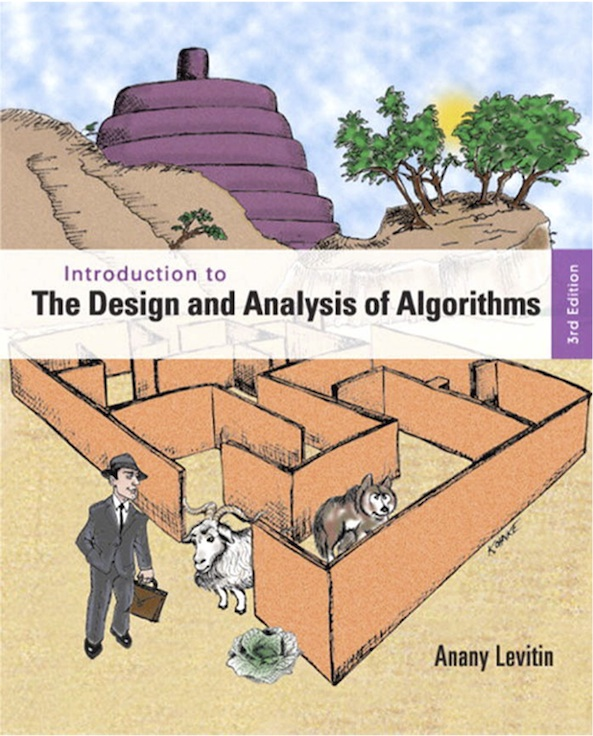
\includegraphics[height=.8\textheight]{img/capa-levitin.jpg}
  \end{center}
  (seção 2.3)
\end{frame}

\section{Um exemplo introdutório}

\begin{frame}
  \frametitle{Exemplo}

  \begin{example}[Busca do maior elemento em uma sequência]
    \begin{codebox}
\Procname{$\proc{Max-Item}(A)$}
\li $\id{max} \gets A[1]$
\li \For $i \gets 2$ \To $\id{length}[A]$
\li \Do
      \If $A[i] > \id{max}$
\li   \Then
        $\id{max} \gets A[i]$
      \End    
    \End    
\li \Return $\id{max}$
\end{codebox}

  \end{example}
\end{frame}

\begin{frame}
  \frametitle{Exemplo}

  \begin{small}
    \begin{codebox}
\Procname{$\proc{Max-Item}(A)$}
\li $\id{max} \gets A[1]$
\li \For $i \gets 2$ \To $\id{length}[A]$
\li \Do
      \If $A[i] > \id{max}$
\li   \Then
        $\id{max} \gets A[i]$
      \End    
    \End    
\li \Return $\id{max}$
\end{codebox}

  \end{small}

\begin{itemize}
\item Tamanho da entrada: $\id{length}[A]$, digamos $n$.
\item Operações mais executadas: corpo do $\For$.
  \begin{itemize}
    \item A comparação é executada mais vezes que a atribuição
    \item A comparação $A[i] > \id{max}$ é a \emph{operação básica}
    \item O número de comparações
      executadas é o mesmo para
      qualquer entrada de tamanho
      $n$
      
      \alert{$\Longrightarrow$}
      Não precisa estudar pior caso, caso médio, nem melhor caso.
  \end{itemize}
  \end{itemize}
\end{frame}


\begin{frame}
  \frametitle{Exemplo}

  \begin{small}
    \begin{codebox}
\Procname{$\proc{Max-Item}(A)$}
\li $\id{max} \gets A[1]$
\li \For $i \gets 2$ \To $\id{length}[A]$
\li \Do
      \If $A[i] > \id{max}$
\li   \Then
        $\id{max} \gets A[i]$
      \End    
    \End    
\li \Return $\id{max}$
\end{codebox}

  \end{small}

Seja $C(n)$ o número de comparações realizadas.
\begin{itemize}
\item A cada iteração, é realizada uma (1) comparação.
\item $C(n) = \sum_{i=2}^{n} 1 = n - 2 + 1 = n - 1 \in \Theta(n) $.
\item (resultado esperado)
\end{itemize}
\end{frame}

\section{Estratégia de análise}

\begin{frame}
\frametitle{Estratégia para analizar complexidade de algoritmos não recursivos}

\begin{enumerate}
\item Escolher um parâmetro (ou vários) para indicar o tamanho da entrada
\item Identificar a operação básica do algoritmo
\item Verificar se o número de vezes que a operação básica é executada depende apenas do tamanho da entrada

\alert{$\Rightarrow$} Caso contrário, o pior caso, o caso médio e o melhor caso devem ser aferidos individualmente
\item Escreva um somatório que expressa quantas vezes a operação básica é executada
\item Usando as leis da aritmética, encontre uma formulação que só depende de $n$, ou pelo menos o seu crescimento asintótico.
\end{enumerate}

\end{frame}

\begin{frame}
\frametitle{Propriedades importantes}

\begin{eqnarray*}
\sum_{i=L}^U \left(c \times a_i\right) & = & c \times \left(\sum_{i = L}^U a_i \right) \\
\sum_{i=L}^U \left(a_i \pm b_i\right) & = & \left(\sum_{i = L}^U a_i \right) \pm \left(\sum_{i = L}^U b_i \right) \\
\sum_{i=L}^U 1 & = & U - L + 1 \\
\sum_{i=1}^n i & = & \frac{n\times (n+1)}{2} \approx \frac{1}{2}\times n^2 \in \Theta(n^2)
\end{eqnarray*}

\end{frame}

\section{Um segundo exemplo}
\begin{frame}
\frametitle{Um segundo exemplo}
\begin{example}[Teste de unicidade dos elementos]
\begin{codebox}
\Procname{$\proc{Unicity-Elems}(A)$}
\li \For $i \gets 1$ \To $\id{length}[A]-1$
\li \Do
      \For $j \gets i+1$ \To $\id{length}[A]$
\li   \Do
        \If $A[i] = A[j]$
\li     \Then
          \Return $\const{False}$
        \End    
      \End    
    \End    
\li \Return $\const{True}$
\end{codebox}

\end{example}
\end{frame}

\begin{frame}
\frametitle{Aplicação da estratégia}

\begin{small}
\begin{codebox}
\Procname{$\proc{Unicity-Elems}(A)$}
\li \For $i \gets 1$ \To $\id{length}[A]-1$
\li \Do
      \For $j \gets i+1$ \To $\id{length}[A]$
\li   \Do
        \If $A[i] = A[j]$
\li     \Then
          \Return $\const{False}$
        \End    
      \End    
    \End    
\li \Return $\const{True}$
\end{codebox}

\end{small}

\begin{enumerate}
\item O tamanho da entrada é o número de elementos de $A$, digamos $n$.
\item O laço mais interno contem um teste de igualdade. A operação básica é o \emph{teste de igualdade}.
\item O número de testes efetuados não depende só de $n$, mas também do
  conteúdo de $A$. Mas precisamente se tem elementos iguais, e quais
  posições eles ocupam.

  Vamos nos interessar à complexidade \alert{no pior caso}: $C_{\textit{pior}}(n)$.
\end{enumerate}
\end{frame}

\begin{frame}
\frametitle{Aplicação da estratégia}

\begin{small}
\begin{codebox}
\Procname{$\proc{Unicity-Elems}(A)$}
\li \For $i \gets 1$ \To $\id{length}[A]-1$
\li \Do
      \For $j \gets i+1$ \To $\id{length}[A]$
\li   \Do
        \If $A[i] = A[j]$
\li     \Then
          \Return $\const{False}$
        \End    
      \End    
    \End    
\li \Return $\const{True}$
\end{codebox}

\end{small}

O pior caso é quando o número de comparações é o maior possível.
\begin{enumerate}
\item ou todos os elementos são distintos dois a dois;
\item ou apenas os elementos nas últimas duas posições são iguais.
\end{enumerate}
\begin{eqnarray*}
C_{\textit{pior}}(n) & = & \sum_{i = 1}^{n-1} \sum_{j = i+1}^{n} 1
\end{eqnarray*}
\end{frame}

\begin{frame}
\frametitle{Aplicação da estratégia}

\begin{small}
\begin{codebox}
\Procname{$\proc{Unicity-Elems}(A)$}
\li \For $i \gets 1$ \To $\id{length}[A]-1$
\li \Do
      \For $j \gets i+1$ \To $\id{length}[A]$
\li   \Do
        \If $A[i] = A[j]$
\li     \Then
          \Return $\const{False}$
        \End    
      \End    
    \End    
\li \Return $\const{True}$
\end{codebox}

\end{small}

\begin{eqnarray*}
C_{\textit{pior}}(n) & = & \sum_{i = 1}^{n-1} \sum_{j = i+1}^{n} 1 \pause = \sum_{i=1}^{n-1} n - (i+1) + 1 \pause = \sum_{i=1}^{n-1} n - i \pause \\
& = & \sum_{i=1}^{n-1} n - \sum_{i=1}^{n-1} i \pause = (n-1)\times n - \frac{(n-1)\times n}{2} \pause \\
& = & \frac{(n-1)\times n}{2} \pause \approx \frac{1}{2}\times n^2 \pause \in \Theta(n^2)
\end{eqnarray*}
\end{frame}

\section{Um terceiro exemplo}
\begin{frame}
\frametitle{Um terceiro exemplo}
\begin{example}{Multiplicação de duas matrizes quadradas}
\begin{codebox}
\Procname{$\proc{Mult-Matrix}(A, B, C)$}
\li \For $i \gets 1$ \To $\id{NbLines}[A]$
\li \Do
      \For $j \gets 1$ \To $\id{NbCols}[B]$
\li   \Do
        $C[i,j] \gets 0$
\li     \For $k \gets 1$ \To $\id{NbCols}[A]$
\li     \Do
        $C[i,j] \gets C[i,j] + A[i, k] \times B[k, j]$
        \End    
      \End    
    \End    
\end{codebox}

\end{example}
\end{frame}

\begin{frame}
\frametitle{Aplicação da estratégia}

\begin{small}
\begin{codebox}
\Procname{$\proc{Mult-Matrix}(A, B, C)$}
\li \For $i \gets 1$ \To $\id{NbLines}[A]$
\li \Do
      \For $j \gets 1$ \To $\id{NbCols}[B]$
\li   \Do
        $C[i,j] \gets 0$
\li     \For $k \gets 1$ \To $\id{NbCols}[A]$
\li     \Do
        $C[i,j] \gets C[i,j] + A[i, k] \times B[k, j]$
        \End    
      \End    
    \End    
\end{codebox}

\end{small}

\begin{itemize}
\item Tamanho (digamos $n$): ordem das matrizes $A$, $B$, $C$.

  Obs. número de elementos $m$ das matrizes é tal que $m = n^2$.
\item Operação básica (laço mais aninhado): 1 adição + 1 multiplicação. 
\end{itemize}
\begin{eqnarray*}
M(n) & = & \sum_{i=1}^n \sum_{j=1}^{n} \sum_{k=1}^n 1 = \sum_{i=1}^n \sum_{j=1}^{n} n = \sum_{i=1}^n n^2 = n^3. 
\end{eqnarray*}
\end{frame}

\section{Um exemplo não tão simlpes}
\begin{frame}
\frametitle{Um exemplo não tão simples}
\begin{example}{Tamanho da representação binária de um inteiro}
\begin{codebox}
\Procname{$\proc{Binary}(n)$}
\li $\id{count} \gets 1$
\li \While $n > 1$
\li \Do
      $\id{count} \gets \id{count}+1$
\li   $n \gets \lfloor n/2 \rfloor$
    \End    
\li \Return $\id{count}$
\end{codebox}

\end{example}
\end{frame}

\begin{frame}
\frametitle{Aplicação da estratégia}
\begin{footnotesize}
\begin{codebox}
\Procname{$\proc{Binary}(n)$}
\li $\id{count} \gets 1$
\li \While $n > 1$
\li \Do
      $\id{count} \gets \id{count}+1$
\li   $n \gets \lfloor n/2 \rfloor$
    \End    
\li \Return $\id{count}$
\end{codebox}

\end{footnotesize}
\begin{itemize}
\item A entrada é um inteiro $n$. O tamanho da entrada é o próprio $n$.
\item A operação executada mais vezes é a comparação $n > 1$. É igual
ao número de vezes que o laço é executado mais um.
\item $n$ apenas recebe alguns valores da faixa formada pelos seus valores
  inicial e final.
\item O valor de $n$ é dividido a cada iteração. 
\item O número de vezes qua operação básica é executada é $\lfloor \log_2 n \rfloor + 1$.
\item Utilizaremos uma \alert{relação de recorrência} para mostrar isto.
\end{itemize}
\end{frame}

\section{Prática}

\begin{frame}
\frametitle{Variação de amostra}

\begin{problem}[Cálculo de variação de amostra]
\begin{eqnarray*}
\mathcal{V}(x_1 \cdots x_n) & = & \frac{\sum_{i=1}^{n} (x_i - \bar{x})^2}{n-1}
\mbox{ onde } \bar{x} = \frac{\sum_{i=1}^{n} x_i}{n} \\
& = & \frac{\sum_{i=1}^n x_i^2 - (\sum_{i=1}^n x_i)^2/n}{n-1}.
\end{eqnarray*}
Encontre e compare a quantidade de cada tipo de operação para calcular a
variação de amostra com cada uma das fórmulas.
\end{problem}
\end{frame}

\begin{frame}
\frametitle{Análise de algoritmo 1}

\begin{problem}
\begin{codebox}
\Procname{$\proc{Mystery-1}(n)$}
\li $s \gets 0$
\li \For $i \gets 1$ \To $n$
    \Do
\li   $s \gets s + i \times i$
    \End
\li \Return $s$
\end{codebox}
\begin{enumerate}
\item O que este algoritmo calcula?
\item Qual a sua operação básica? Quantas vezes é executada?
\item Qual a classe de complexidade do algoritmo?
\item Existe um algoritmo mais eficiente? Se existir, qual a classe de complexidade dele? Senão, porque?
\end{enumerate}
\end{problem}
\end{frame}

\begin{frame}
\frametitle{Análise de algoritmo 2}

\begin{problem}
\begin{codebox}
\Procname{$\proc{Mystery-2}(A)$}
\li $m_1 \gets A[1]$, $m_2 \gets A[1]$
\li \For $i \gets 2$ \To $\id{length}[A]$
\li \Do
      \If $A[i] < m_1 \kw{then}\, m_1 \gets A[i]$
\li   \If $A[i] > m_2 \kw{then}\, m_2 \gets A[i]$
    \End
\li \Return $m_2 - m_1$
\end{codebox}
\begin{enumerate}
\item O que este algoritmo calcula?
\item Qual a sua operação básica? Quantas vezes é executada?
\item Qual a classe de complexidade do algoritmo?
\item Existe um algoritmo mais eficiente? Se existir, qual a classe de complexidade dele? Senão, porque?
\end{enumerate}
\end{problem}
\end{frame}

\begin{frame}
\frametitle{Análise de algoritmo 3}

\begin{problem}
\begin{codebox}
\Procname{$\proc{Mystery-3}(A)$}
\li \For $i \gets 1$ \To $\id{NbLines}[A]-1$
\li \Do
      \For $j \gets i+1$ \To $\id{NbLines}[A]$
\li   \Do
        \If $A[i,j] \neq A[j,i]$ \kw{then} \Return $\const{False}$
      \End
    \End
\li \Return $\const{True}$
\end{codebox}
\begin{enumerate}
\item O que este algoritmo calcula?
\item Qual a sua operação básica? Quantas vezes é executada?
\item Qual a classe de complexidade do algoritmo?
\item Existe um algoritmo mais eficiente? Se existir, qual a classe de complexidade dele? Senão, porque?
\end{enumerate}
\end{problem}
\end{frame}


\end{document}
